\documentclass{beamer}
\usepackage{graphicx}
\usepackage{verbatim} % For using /begin{comment}; /end{comment}

\definecolor{oj}{rgb}{1.0,0.65,0.0}
\definecolor{cblue}{rgb}{0.39,0.58,0.93}


\setbeamercolor{normal text}{bg=black, fg=white}
\setbeamercolor{title}{fg=oj}
\setbeamercolor{frametitle}{fg=oj}
\setbeamercolor{block title}{fg=green}
\setbeamercolor{itemize item}{fg=cblue} % all frames will have red bullets
\setbeamercolor{enumerate item}{fg=cblue} % all frames will have red bullets

\usefonttheme{serif}
\setbeamerfont{frametitle}{series=\bfseries} % Frame titles should be bold

\title{Coronal Seismology}
\subtitle{ASTR 598}
\date{Spring 2016}
\author{Laurel Farris}

\begin{document}

\begin{frame}
    \titlepage
\end{frame}

\begin{frame}{Overview}
    The body of the frame
\end{frame}

\begin{frame}{Kinks and Sausages}
    \begin{figure}
        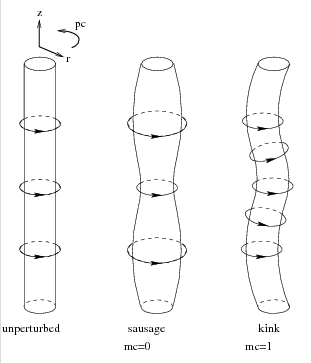
\includegraphics[width=3in]{kink_saus.png}
    \caption*{\tiny image credit:
    $https://inspirehep.net/record/1088737/files/figures_instab_locations.png$}
    \end{figure}
\end{frame}

\begin{frame}{Kink modes}
    In general $\ldots$
    \begin{itemize}
        \item fast magnetoacoustic waves
        \item m = 1
        \item low plasma $\beta$
        \item present in coronal loops
    \end{itemize}
\end{frame}

\begin{frame}{Damping profiles of kink waves}
    \begin{itemize}
        \item Gaussian vs. exponential
        \item Plasma motions around footpoints of coronal loops
    \end{itemize}
\end{frame}

\begin{frame}{Sausage modes}
\end{frame}

\begin{frame}{My Research}
\end{frame}

\end{document}
